\documentclass[12pt,a4paper,final,twoside,openright]{report}
\usepackage[utf8]{inputenc}
\usepackage[T1]{fontenc}
\usepackage[catalan]{babel}

\usepackage{setspace}
\onehalfspacing

\usepackage{graphicx}
\usepackage{caption}
\usepackage{amsmath}
\usepackage{hyperref}

\usepackage{epstopdf}

\usepackage[left=2.5cm,right=2.5cm,top=2.5cm,bottom=2.5cm]{geometry}

\usepackage{fancyhdr}
\pagestyle{fancy}
\fancyhead{}
\fancyhead[RO,LE]{\thepage}
\fancyhead[RE,LO]{Control d'un doble integrador}
\fancyfoot{}
\fancyfoot[RO,LE]{
\includegraphics[scale=0.5]{Imatges/etseib.png}}


\usepackage{appendix}
\renewcommand{\appendixname}{Annexos}
\renewcommand{\appendixtocname}{Annexos}
\renewcommand{\appendixpagename}{Annexos}


\usepackage{chngcntr}
\counterwithin{figure}{chapter}%Permet que el comptatge de les figures sigui segons capitol
\counterwithin{table}{chapter}
\counterwithin{equation}{chapter}
\counterwithin{footnote}{chapter}

%PLANTEJAR TEMA DE \autoref{} ja que així l'hiperenllaç es també per la paraula i no sols el numero.

\renewcommand{\thefigure}{\arabic{chapter}.\arabic{figure}}
\renewcommand{\thetable}{\arabic{chapter}.\arabic{table}}
\renewcommand{\theequation}{\arabic{chapter}.\arabic{equation}}
\renewcommand{\thefootnote}{\arabic{footnote}}

\usepackage{etoolbox}
\usepackage{subcaption}
\patchcmd{\chapter}{\thispagestyle{plain}}{\thispagestyle{fancy}}{}{}

\headheight = 15pt %Donava un warning sino

\textheight = 690pt %Col·locació de l'escut a distancia que quedi be
\footskip = 60pt

\usepackage{enumitem}

\graphicspath{{Imatges/}}
\usepackage{color}

\usepackage{multirow}
\newcommand{\specialcell}[2][c]{%
  \begin{tabular}[#1]{@{}c@{}}#2\end{tabular}}

\title{Tecnologia de Control \\ Identificació i control d'un motor}
\author{Alumne: Lluís Salord Quetglas \\ Professor: Manel Velasco}
\date{Gener 2016}

\begin{document}

\maketitle
\thispagestyle{empty}

\cleardoublepage

\setcounter{page}{1} %Començar en la pagina 1

\begin{abstract}
\addcontentsline{toc}{chapter}{Resum}
alksfj klañjds klañjsdfkljwqeriojgd odjfs alskdf alksfj klañjds klañjsdfkljwqeriojgd odjfs alskdf alksfj klañjds klañjsdfkljwqeriojgd odjfs alskdf alksfj klañjds klañjsdfkljwqeriojgd odjfs alskdf alksfj klañjds klañjsdfkljwqeriojgd odjfs alskdf alksfj klañjds klañjsdfkljwqeriojgd odjfs alskdf alksfj klañjds klañjsdfkljwqeriojgd odjfs alskdf alksfj klañjds klañjsdfkljwqeriojgd odjfs alskdf alksfj klañjds klañjsdfkljwqeriojgd odjfs alskdf alksfj klañjds klañjsdfkljwqeriojgd odjfs alskdf alksfj klañjds klañjsdfkljwqeriojgd odjfs alskdf alksfj klañjds klañjsdfkljwqeriojgd odjfs alskdf alksfj klañjds klañjsdfkljwqeriojgd odjfs alskdf alksfj klañjds klañjsdfkljwqeriojgd odjfs alskdf 
\end{abstract}

\tableofcontents

\listoffigures

%\listoftables

\chapter{Introducció}

En aquesta segona part del curs es pretenen aconseguir dos objectius principals. Per una banda, la identificació d'un model aproximat d'un motor que presenta un comportament no-lineal. Per altra banda, dur a terme el control de forma eficient del motor presentat. A continuació es fa una breu explicació dels dispositius utilitzats per portar a terme aquests objectius per tal de facilitar la comprensió del nucli de l'informe, la identificació i la implementació del control.

El primer a descriure és el motor. Aquest és un motor EMG30 de 12 V que porta dos \textit{encoders}, se'ls anomena \textit{encoder A} i \textit{encoder B} al llarg de l'informe, aquests donen en total 360 polses/revolució. Per tant, aquests permeten extreure la posició del motor, amb el coneixement del sentit de gir, o la velocitat si es té la diferència de temps entre polses. S'ha de tenir en compte que internament el motor porta un reductor de 30:1, per tant, els polses per revolució de l'eix exterior del motor és de 1080 polses/revolució. 

Entre el motor i l'Arduino es troba una placa que permet dur a terme el control del motor amb l'Arduino. En aquesta, entre d'altres coses conté dos circuits integrats que controlen els \textit{H-bridge} per dos canals diferents, A i B, permetent així amb una mateixa placa controlar dos motors diferents. El circuit \textit{H-bridge} permet el canvi de sentit del motor, segons el valor d'una senyal. 

Per tant, es pot canviar el sentit de gir, però no es sap realment en quin sentit està anant. Per saber-ho el que es fa és observar els valors dels \textit{encoders}. Aquests valors s'han d'observar en el flanc de baixada, ara bé, es pot fer en el l'\textit{encoder A}, en el de l'\textit{encoder B} o dels dos.

\begin{itemize}
\item \textbf{Encoder A}: si els valors dels dos \textit{encoders} són iguals va a dretes.
\item \textbf{Encoder B}: si els valors dels dos \textit{encoders} són diferents va a dretes.
\item \textbf{Encoder A i B}: pren el sentit segons la baixada sigui d'un o altra.
\end{itemize}

Aquesta peculiaritat de saber el sentit de gir es pot utilitzar per saber la posició del motor. Si s'imagina que per cada pols donat en un sentit es suma 1 a un comptador i per cada pols en l'altre sentit es resta 1, s'aconsegueix una mesura de la posició exacte. En aquest cas, si s'utilitzen els dos \textit{encoders} s'aconsegueix una precisió més gran. Per tant, si s'implementen interrupcions per flanc de baixada als ports dels \textit{encoders} es pot dur a terme la mesura de la posició real. Els ports que permeten aquestes interrupcions són el 2 i el 3 de l'Arduino i s'han de configurar com a tal per fer-ho. El primer a fer en la configuració és posar els pins com a entrada i activar els \texttt{Pull-up resistors}. Posteriorment s'han d'activar les interrupcions donant la \texttt{ISR} (Interrupt Service Routines) que ha de fer per tractar la interrupció, en aquest cas la funció \texttt{updateStadistic}. Per tant, les comandes a posar en el \texttt{setup} de l'Arduino serien les següents:

\begin{verbatim}
pinMode(encoder,INPUT); //inputs
pinMode(encoder,INPUT_PULLUP);//Enable pull up resistor
attachInterrupt(digitalPinToInterrupt(encoder),updateStadistic,FALLING);
\end{verbatim} 

Per altra banda, també es possible el càlcul de la velocitat real ja que també amb l'ús de les interrupcions explicades a sobre es pot fer extreure el temps entre polsos. Per tant, si es té el temps entre polsos i la informació dels polses per revolució, amb la formula \eqref{eq:formulaVelocitat} es pot extreure la velocitat instantània del motor. Per donar robustesa al càlcul es pren com a velocitat del motor la mitja de tres mostres.

\begin{equation}\label{eq:formulaVelocitat}
v [RPM] = \frac{2\cdot 10^6}{\triangle t [ms]}
\end{equation}

%Referenciar GitHub i fer-lo

\chapter{Identificació del motor}

La identificació consisteix en trobar un model matemàtic que descrigui el comportament dinàmic de la planta, en aquest cas el motor. D'aquesta forma, si es té un model del motor es pot dur a terme un control amb observador, que és l'objectiu final d'aquesta pràctica (juntament amb l'aprenentatge dels propis alumnes). 

Per extreure aquest model matemàtic, a les classes, s'han plantejat dos mètodes diferents, explicats a continuació:
\begin{enumerate}[label=\textbf{\alph*)}]
\item \textbf{Identification Toolbox}

Aquestes són un conjunt d'eines que permeten la identificació d'un model, donades les dades de les entrades i la sortida corresponent. El problema d'aquest mètode és que el model és com una caixa negre que no es sap que representa cada valor i, per tant, amb falta de significat per l'usuari. Per això, s'ha considerat poc didàctica i no s'ha arribat a utilitzar.

\item \textbf{fminsearch}

En aquest cas, el \texttt{fminsearch} és una funció que busca el mínim d'una funció donada, modificant les variables d'aquesta. Per tant, partint que es té una model teòric del motor, representat per \eqref{eq:model_teoric1} i \eqref{eq:model_teoric2}, les variable a modificar serien els paràmetres del model (\textit{J},\textit{b},\textit{K},\textit{R},\textit{L}) i la funció a minimitzar seria la distància entre \textit{y} de les dades i la \textit{y} del model amb les variables modificades, utilitzant ambdós les mateixos \textit{inputs}.

\begin{eqnarray}
&\frac{d}{dt}\begin{bmatrix}
\dot{\theta}\\
i
\end{bmatrix} = \begin{bmatrix}
-\frac{b}{J} & \frac{K}{J}\\
-\frac{K}{L} & -\frac{R}{L}
\end{bmatrix}
\begin{bmatrix}
\dot{\theta}\\
i
\end{bmatrix} + \begin{bmatrix}
0\\
\frac{1}{L}
\end{bmatrix} V \label{eq:model_teoric1}\\
&y = \begin{bmatrix}
1 & 0
\end{bmatrix} \begin{bmatrix}
\dot{\theta}\\
i
\end{bmatrix}\label{eq:model_teoric2}
\end{eqnarray}
\end{enumerate}

Ara bé, per poder dur a terme aquesta identificació del model, primer s'ha d'assegurar que el sistema és lineal entre l'acció de control, que seria la velocitat desitjada, i la sortida, la velocitat real. Fins i tot en aquest cas, es vol tenir un guany en estacionari de 1, per tant que la velocitat real sigui igual a la desitjada. Actualment, amb l'acció de control que es dona a través del \texttt{PWM} la relació amb la sortida és no-lineal, com es pot observar més endavant en la figura \ref{fig:PWM(vel)}. Per tant, s'ha de fer un procés de linealització del sistema.

\section{Linealització del sistema}

A l'hora de portar a terme la linealització d'un sistema es poden implementar una gran varietat de mètodes que permeten aconseguir-ho. En el primer que es va pensar va ser en l'ús de la idea del \textit{Gain Scheduling}, adaptant el valor d'un controlador $K_c$ segons el valor d'entrada, amb els valors discrets possibles tabulats. Per tant, es crearia una taula amb 255 entrades que donarien la $K_c$ corresponent per cada \texttt{PWM} requerit per donar la velocitat desitjada. Ara bé, aquest mètode, a banda de ser un poc rudimentari, podria arribar a donar problemes de memòria de l'Arduino que està bastant limitat en aquest sentit.

Finalment s'ha decidit per crear una funció que depenent de la velocitat desitjada doni el \texttt{PWM} que hi porta en estacionari. Per fer-ho, s'han extret els valors de la velocitat real, en estacionari, per cadascun dels valors de \texttt{PWM} entre 0 i 255. Matisar que per prendre els valors s'ha esperat un cert temps entre mostra i mostra, per tal que s'agafés el valor en estacionari i, per tant, només influeix el guany estacionari, no la dinàmica. D'aquesta forma es pot extreure una funció aproximada com la representada en \ref{fig:PWM(vel)}.

\begin{figure}[h]
\centering
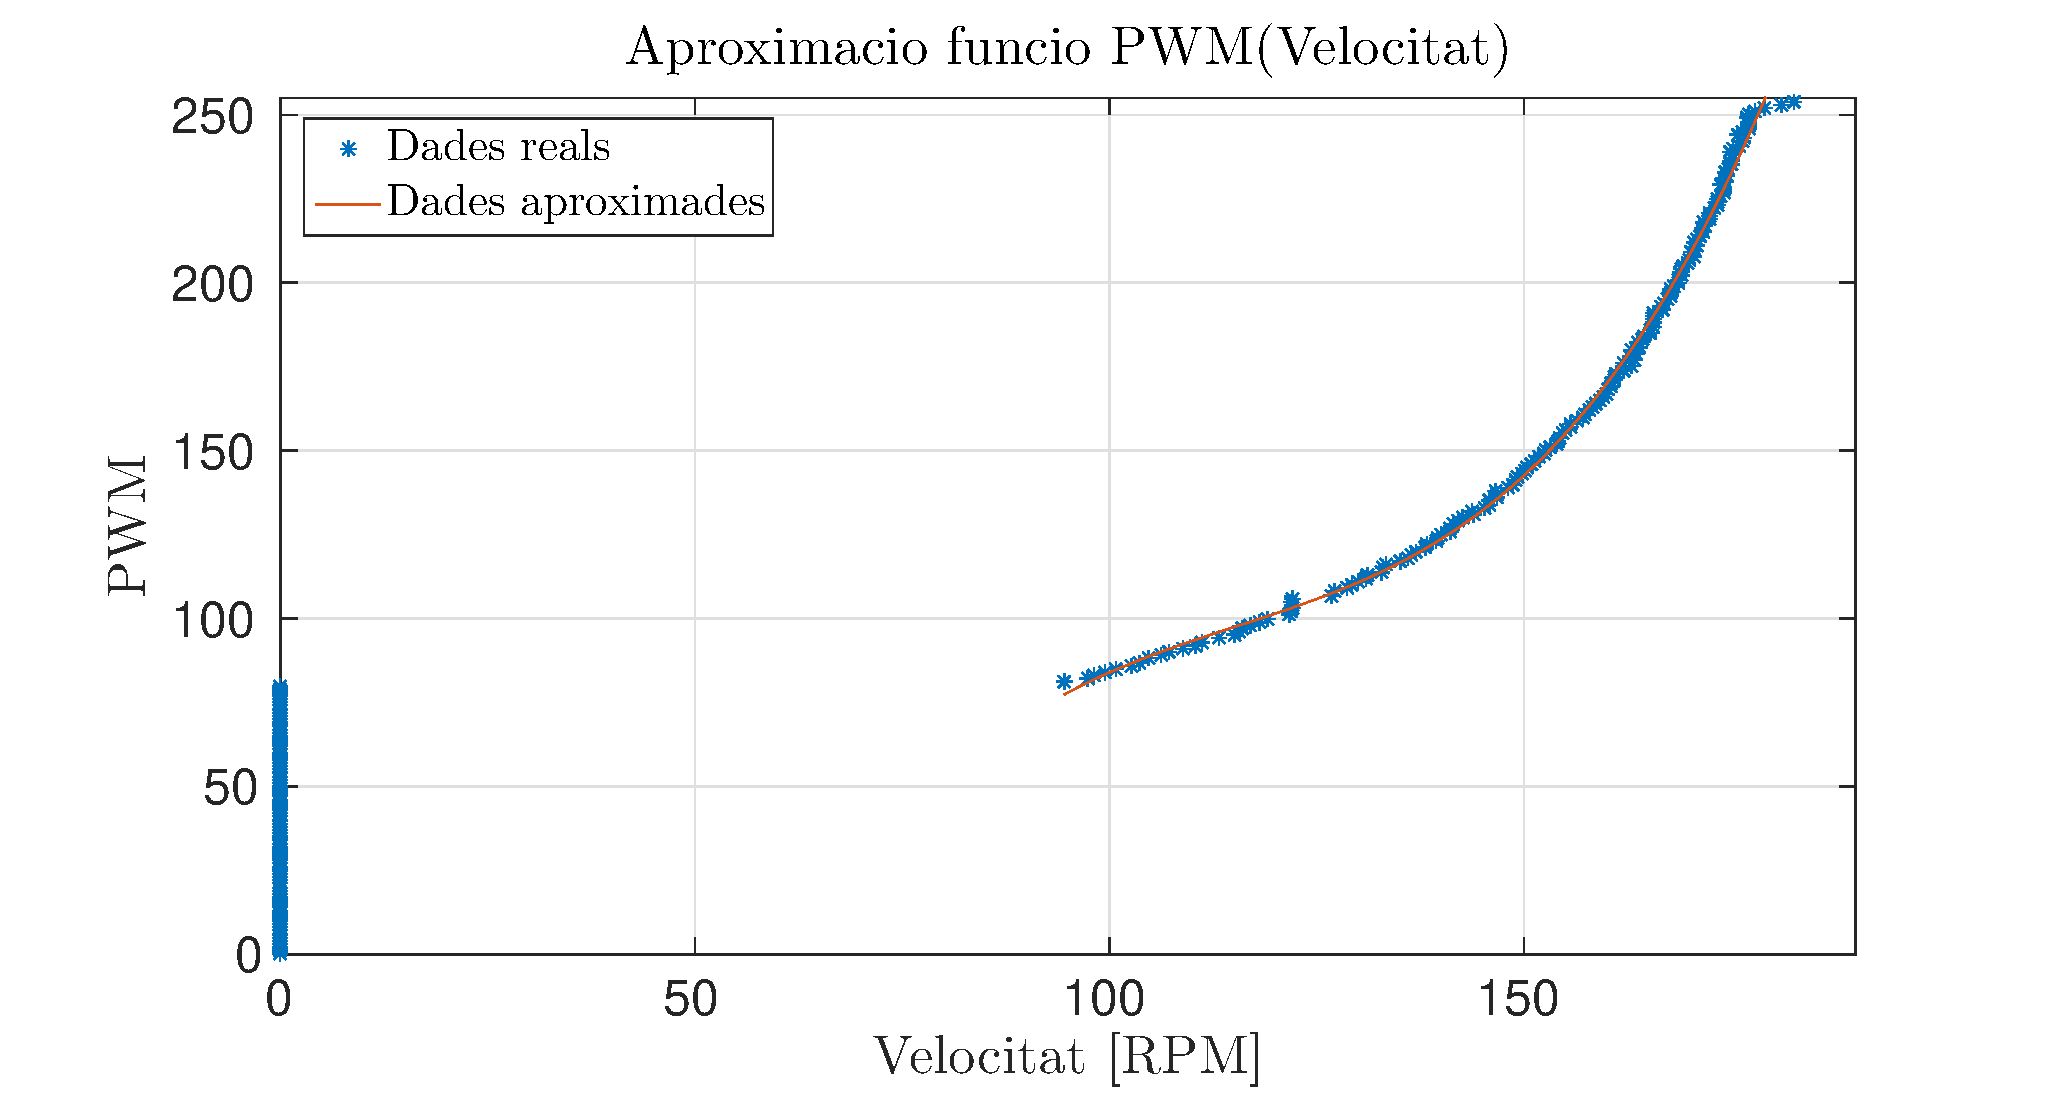
\includegraphics[width=0.8\textwidth]{Imatges/funcioPWM.eps}
\caption{Comparativa i aproximació de la relació entre velocitat i PWM\label{fig:PWM(vel)}}
\end{figure}

Com es pot observar fins un cert \texttt{PWM} el motor no gira, per tant, l'aproximació dels valors s'ha hagut de fer a partir d'aquest valor fins el 255. En aquest cas, l'aproximació, equació \eqref{eq:aprox_PWM(v)} i taula \ref{tab:coef_PWM(v)}, s'ha fet polinòmica i de ordre tres, ja que més gran no s'apreciava pràcticament diferència i tan sols afegeix complexitat. 

\vspace{-10pt}
\begin{equation}\label{eq:aprox_PWM(v)}
PWM(v) = p_1\cdot x^3 + p_2 \cdot x^2 + p_3 \cdot x + p_4
\end{equation}

\begin{table}[h]
\begin{center}
\begin{tabular}{|c|c|c|c|}
\hline
$p_1$ & $p_2$ & $p_3$ & $p_4$\\ \hline
0,0004088 & -0,1414 & 17,1 & -621\\ \hline
\end{tabular}
\caption{Valors dels coeficients de l'aproximació de la funció \textit{PWM(v)}\label{tab:coef_PWM(v)}}
\end{center}
\end{table}

\vspace{-15pt}
Un cop trobada la funció que aproxima el valor del \texttt{PWM} adient per la velocitat desitjada es troba amb el fet que el sistema global de funció i motor, figura \ref{fig:esqSistPWM-Motor}, és pràcticament lineal. Aquest fet es demostra en la figura \ref{fig:linealitat}. Tan sols se'n destaca una zona que no compleix del tot, aparició d'una zona morta, que és al voltant dels 130 RPM, on es manté a la mateixa velocitat real\footnote{Al llarg de la pràctica entre els diferents alumnes no s'ha arribat a una conclusió de perquè és degut.}.

\vspace{-5pt}
\begin{figure}[h]
\centering
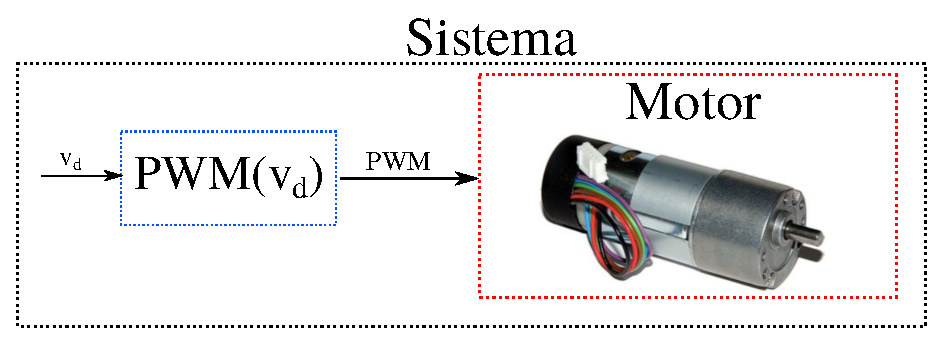
\includegraphics[scale=1]{Imatges/esqPWM-Motor.eps}
\caption{Esquema del funcionament del sistema\label{fig:esqSistPWM-Motor}}
\end{figure}

\begin{figure}[ht]
\centering
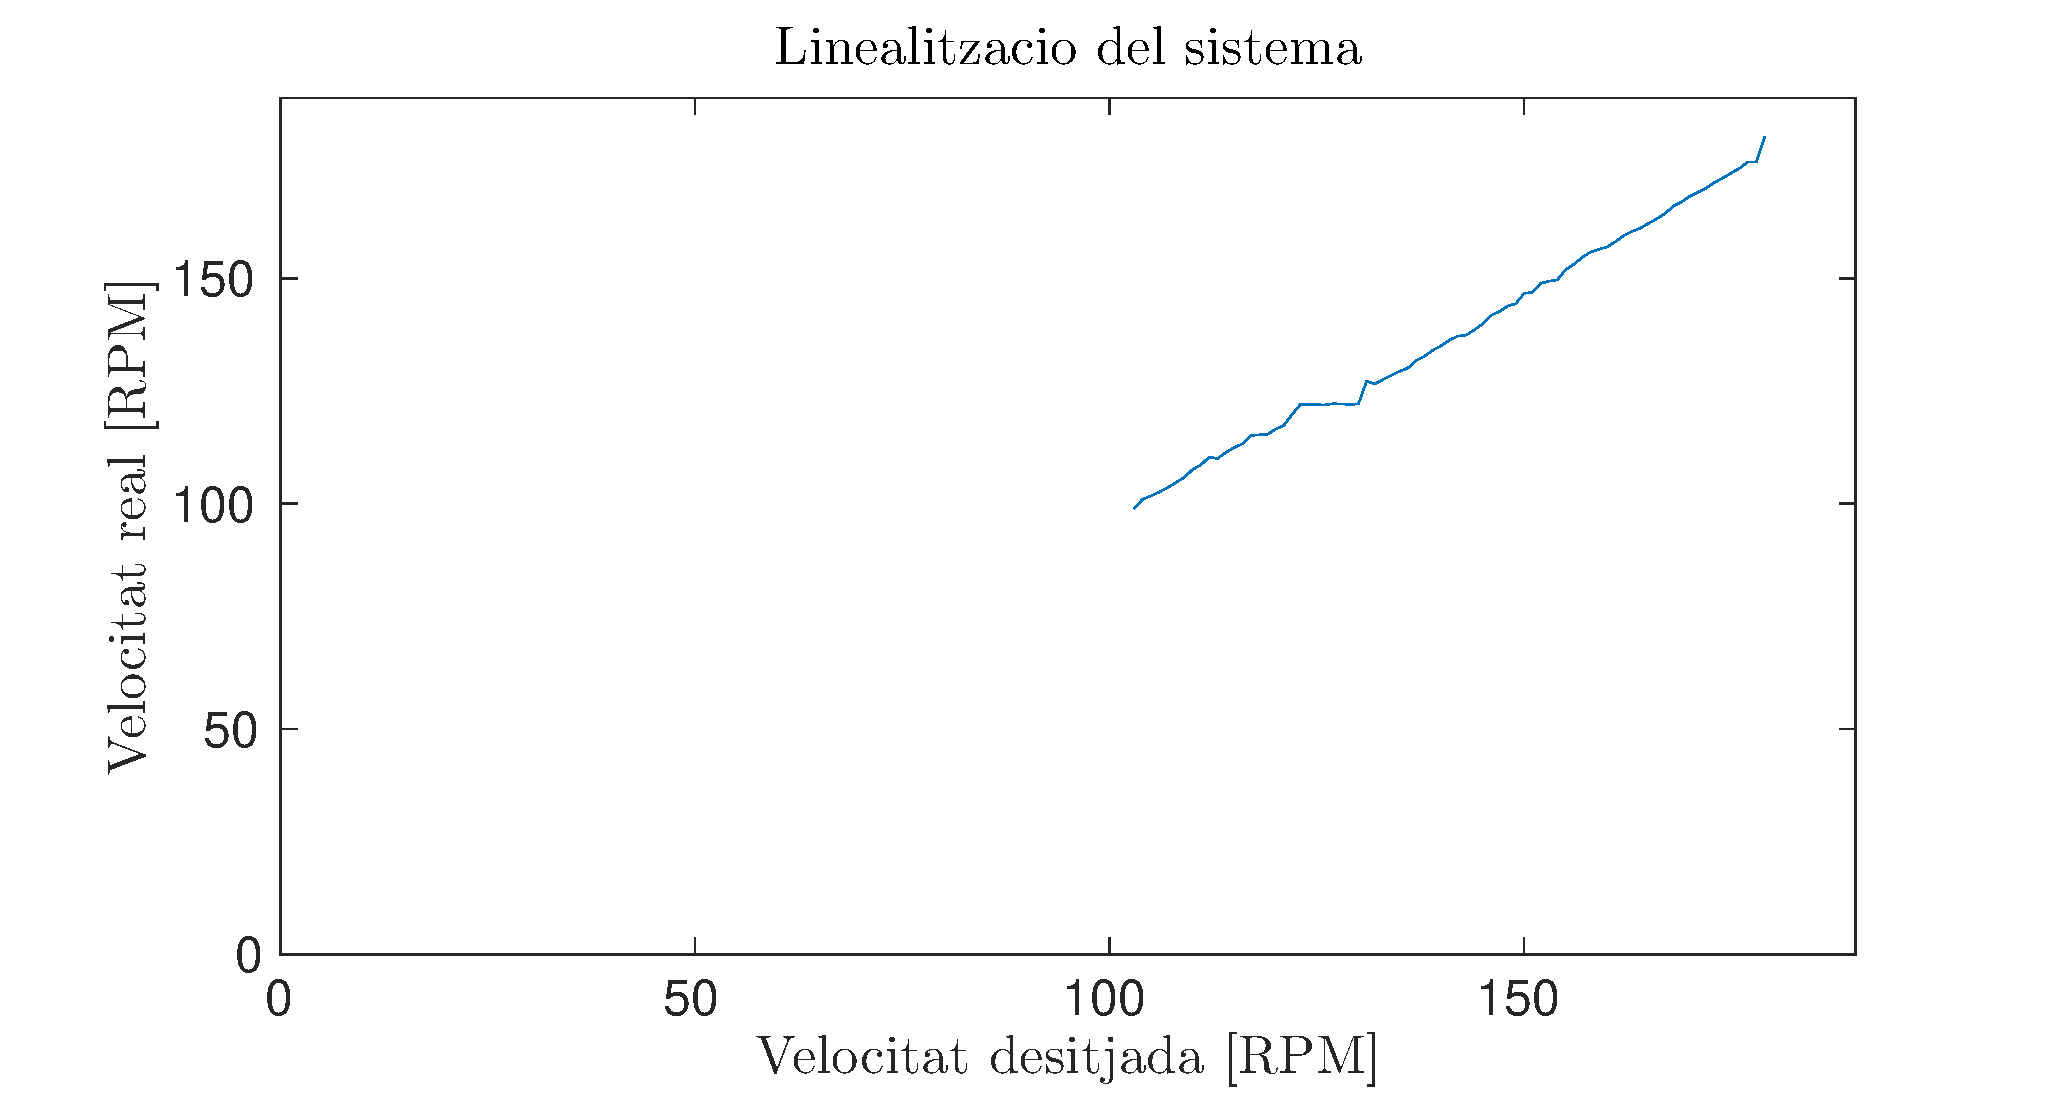
\includegraphics[width=0.8\textwidth]{linealitat.eps}
\caption{Demostració de linealitat entre velocitat desitjada i real\label{fig:linealitat}}
\end{figure}

\section{Extracció del model}
%Acabar d'explicar com funciona el de minimitza una funcio
Un cop s'ha linealitzat el sistema es pot procedir a l'extracció del model que s'havia introduït a l'inici del capítol. Com s'ha explicat anteriorment, s'ha escollit el mètode que minimitza la distància entre la sortida $y$ de les dades i la sortida $y$ del model teòric amb les variables de la funció.

El funcionament en detall és a partir del model matemàtic teòric, \eqref{eq:model_teoric1} i \eqref{eq:model_teoric2}, i les variables (\textit{J},\textit{b},\textit{K},\textit{R},\textit{L}) amb uns valors inicials, es procedeix a la cerca de la mínima distància. Per fer-ho, la funció \texttt{fminsearch} recalcula de forma cíclica la distància i varia els valors seguint alguna \textit{policy} interna, per tal d'arribar al valor mínim.

Un detall a tenir en compte a l'hora de dur a terme l'extracció del model és el fet que com més dades es tinguin més acurat pot arribar a ser el model. Per tant, es desitja dur a terme la presa de mostres amb un temps de mostreig baix, però factible dins els límits de l'Arduino. En aquest cas, s'ha utilitzat un \textit{delay}\footnote{S'hauria pogut utilitzar interrupcions de \textit{Timer} que serien més acurades o, fins i tot, un \textit{Real-Time} per ser-ho més, però no ha donat temps per refer l'experiment.} de $5$ ms, que a la realitat s'aproximava a un temps de mostreig d'uns $6,5$ ms. Destacar el fet que el model s'hagi extret a una certa freqüència no significa que el control s'hagi de fer en aquesta, només serveix per acurar més o menys el model.

\subsection{Restriccions del model}
%Les restriccions com son els parametres positius ja que aquests son fisics i per tant ha de ser positius. I que el sistema es estable, ja que com es pot veure el motor no arriba a explotar.
Ara bé, així com està plantejat el mètode actualment, no es poden tenir en compte una sèrie de fets que no imposa el model teòric, però que en la realitat s'haurien de complir. Per això, es planteja el aquest apartat sobre restriccions que ha de tenir el model que es trobi finalment.

En l'experiència que s'ha tingut amb el motor, s'ha comprovat que en sí aquest és estable, ja que al donar-li una consigna es manté en un valor de forma estacionaria i no s'inestabilitza. Per tant, una restricció que s'ha d'imposar al model, que no és intrínsec del model teòric anterior, és que sigui estable per sí mateix. Això es pot imposar provocant que els valors propis de la matriu $A$, equació \eqref{eq:matriuA}, siguin negatius.

\begin{equation}\label{eq:matriuA}
A = \begin{bmatrix}
-\frac{b}{J} & \frac{K}{J}\\
-\frac{K}{L} & -\frac{R}{L}
\end{bmatrix}
\end{equation}

Per altra banda, el model teòric està basat en paràmetres físics, com són la inèrcia, resistència elèctrica, constants de fricció, etc. Al ser paràmetres físics implícitament han de ser positius, per tant, un model amb valors d'aquests paràmetres negatius seria irreal.

Per tant, s'estableixen com a restriccions del model que sigui estable, o sigui matriu $A$ amb valors propis negatius, i que els paràmetres del model siguin positius. Transformar aquestes restriccions al codi es du a terme mitjançant una condició que imposa en cas de no compliment que el resultat de la distància és igual a infinit. D'aquesta forma la \textit{policy} interna de la funció \texttt{fminsearch} detecta que aquella combinació de paràmetres no és adequada i, per tant, que ha d'anar en una altra direcció.

\subsection{Model final}

A partir del mètode presentat anteriorment, amb les modificacions pertinents per tenir en compte les restriccions comentades, s'ha aconseguit extreure un model matemàtic del motor.

A l'hora de trobar un òptim, degut a la \textit{policy} interna de la funció \texttt{fminsearch}, es depèn del valor inicial dels paràmetres. Al intentar fer-ho el millor possible es van prendre com a valors inicials el d'un motor de característiques similars\footnote{Control Tutorials for Matlab \& Simulink. \textit{DC Motor Speed: System Modeling}. \texttt{http://ctms.engin.umich.edu}}, però pel que sembla amb aquestes l'optimització es queda en bucle en aquests valors ja que qualsevol valor pròxim no compleix les restriccions. Per això, s'ha pres 1 com a valors inicials de tots els paràmetres\footnote{Un possible treball futur podria ser la cerca de paràmetres inicials que portin a valors més realistes.}. En la configuració presentada el resultat de minimització de la distància és el representat a la taula \ref{tab:modelFinal}. 

\begin{table}[h]
\centering
\begin{tabular}{|c|c|c|c|c|}
\hline
$J$ & $b$ & $K$ & $R$ & $L$\\ \hline
0.003340 & 2.892346 & 1.003141 & 0.0001173 & 0.013377 \\ \hline
\end{tabular}
\caption{Valors dels paràmetres del model final\label{tab:modelFinal}}
\end{table}

En el cas d'estudi, la distància no arriba a valor nul, ja que abans d'això dona un error per a poder fer la conversió del model continü a discret (funció \texttt{c2d} del Matlab), i, per tant, el bucle acaba en aquest punt amb el resultat donat anteriorment. Aquest model final s'adapta prou bé a les dades que s'han donat inicialment. Això es pot comprovar de dues formes diferents, per una banda, la distància, del conjunt resultant, és de $282,11$ però aquest repartit entre les $5792$ mostres dona de mitja un error de $0,0019$, per tant, és bastant acurat. Per altra banda, és pot comprovar mitjançant la figura \ref{fig:comp_model_real}, on es veu que en gran mesura els valors coincideixen.

\begin{figure}[h]
\centering
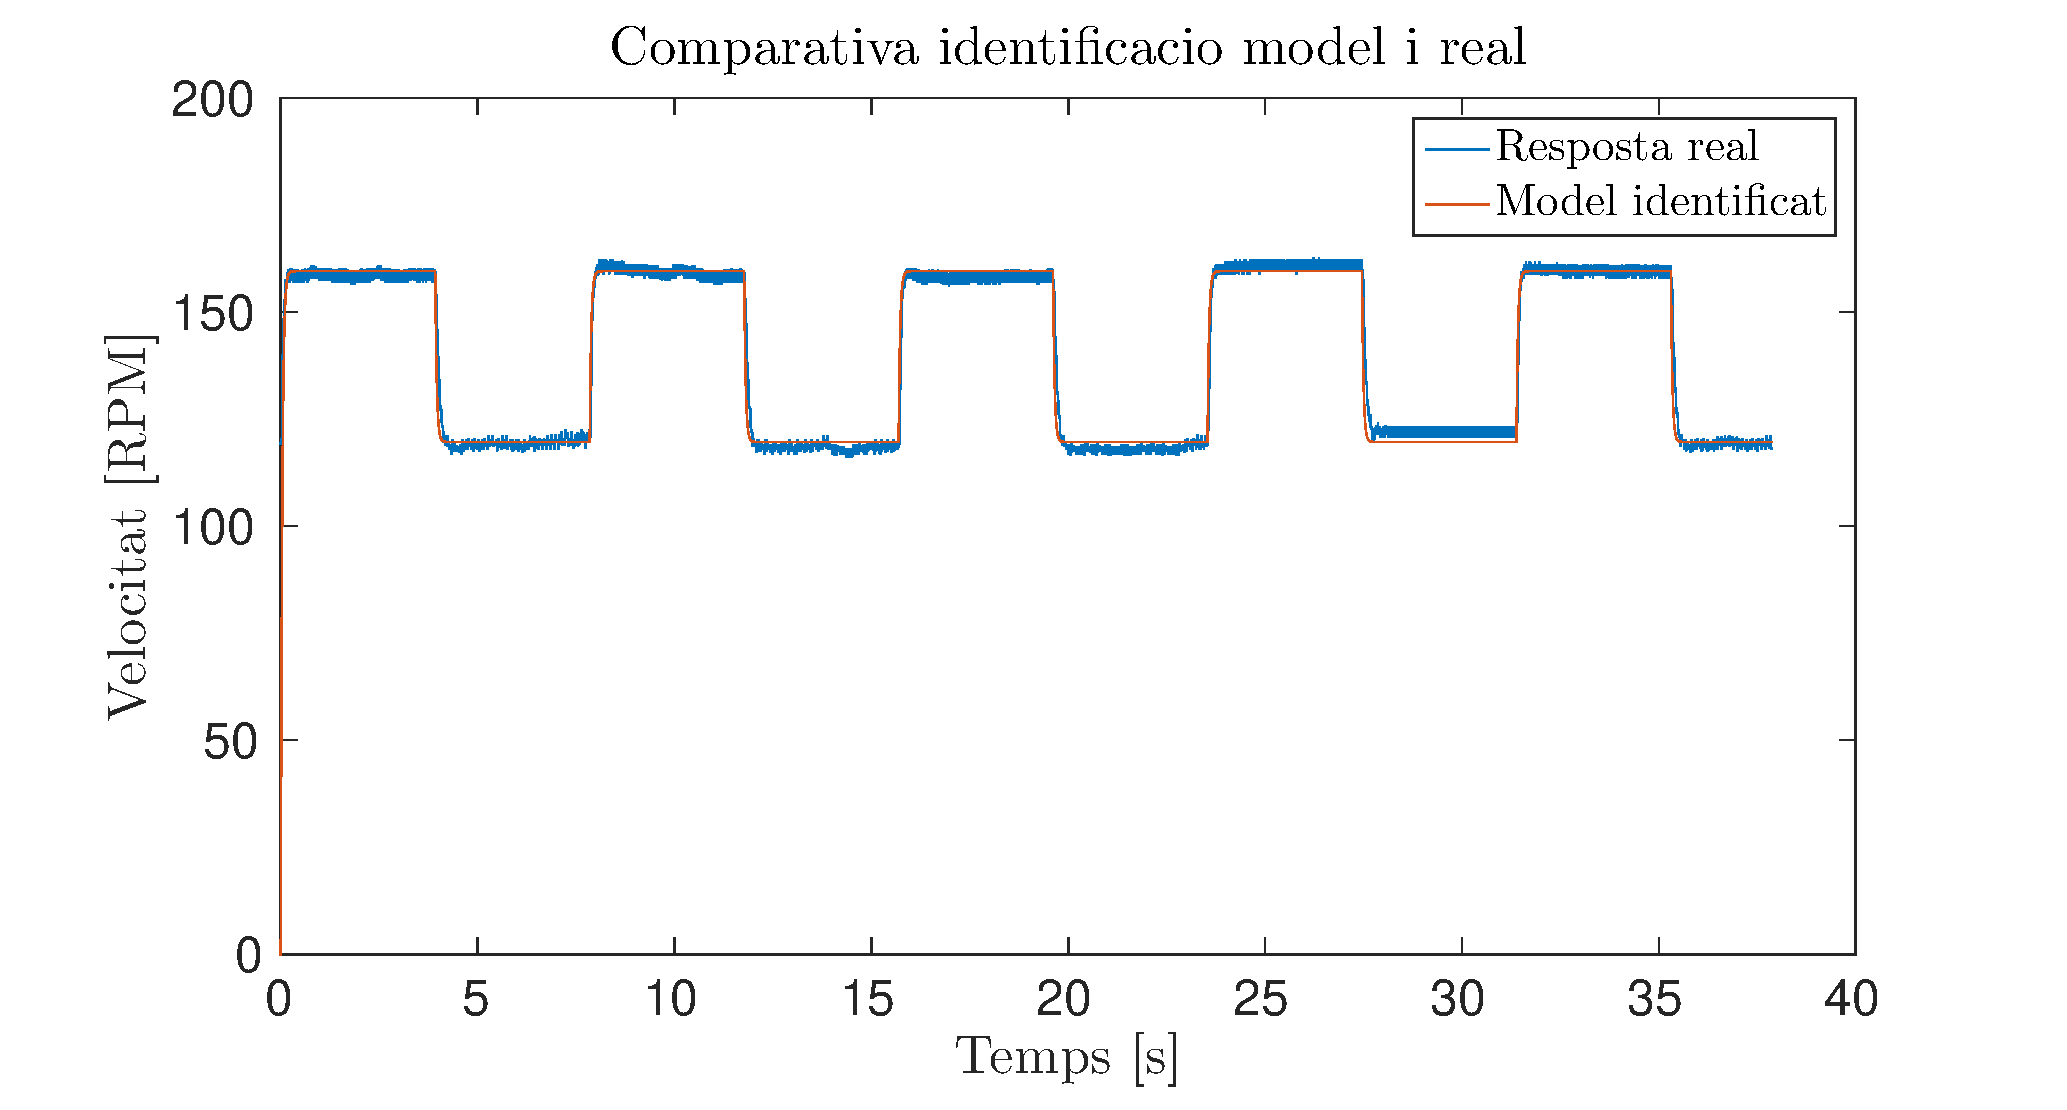
\includegraphics[width=0.8\textwidth]{Imatges/identificacio.eps}
\caption{Comparativa entre el model extret i els valors reals\label{fig:comp_model_real}}
\end{figure}

Finalment, s'ha pogut extreure un model que aproxima prou bé el comportament real del motor. Per tant, al tenir un model de la planta, és pot procedir a dur a terme el control.

\chapter{Control del motor}
El motor amb el que es treballa, com s'ha mencionat anteriorment, se'n pot extreure la velocitat, però també la intensitat i, per tant, amb aquestes variables suposadament es podria dur a terme un control discret per realimentació d'estats. El problema és que la senyal de la intensitat és molt sorollosa, fins i tot, tant que és més recomanable no utilitzar-la. Per tant, si una de les variables d'estat del sistema no pot ser utilitzada directament, l'opció que queda és l'ús d'un control amb observació.

Al haver treballat en el doble integrador amb control amb observació i, fins i tot, amb refús de pertorbacions, en aquest cas, es treballa directament amb el control amb refús de pertorbacions constants. Aquest tipus de control permet suavitzar o, fins i tot, eliminar l'error que pugui tenir el model respecte la realitat. Per tant, a l'hora de dur a terme el control es parteix de la base de codi del doble integrador i s'adapta al cas actual. També, al prendre com a base aquest codi s'ha obviat el dur a terme les simulacions amb Simulink i s'ha treballat directament sobre l'Arduino.

En aquest pràctica tan sols es planteja com a obligatori el control de velocitat del motor, ara bé, si es desitja també es pot mirar de dur a terme el control de posició. En el cas d'estudi, es presenten tant el control de velocitat, com el de posició, tot i que aquest últim no s'hagi aconseguit aplicar en la seva totalitat.

\section{Control de velocitat}

El control de velocitat consisteix en provocar que el motor segueixi les diferents consignes de velocitats que es donin. Per aconseguir-ho, com s'ha dit abans, s'utilitza un control amb observador i refús de pertorbacions constants, amb el model que s'ha extret al capítol anterior. 

Al treballar amb un control amb observador, es requereix d'almenys una variable d'estat. En aquest cas, aquesta és la velocitat de rotació que es pot obtenir a partir d'implementar el que s'ha explicat en la introducció del treball. Si es fan els estudis sobre el model final de controlabilitat, sistema controlable si $\begin{bmatrix}B & AB\end{bmatrix}$ és de rang complert, i d'observabilitat, sistema observable si $\begin{bmatrix}C\\CA\end{bmatrix}$ és de rang complert; és comprova que és controlable i observable i, per tant, que es pot dur a terme el control amb observador. 


A l'hora de dur a terme el control s'utilitzen els càlculs que s'han utilitzat en el control del doble integrador, en la diferència d'un altra model i, per tant, matrius diferents, i de l'ús d'uns pols de llaç tancat, tant de la planta com de l'observador, que s'adaptin al cas d'estudi. La planta que s'ha extret del té uns pols de llaç obert molt negatius, per tant, molt ràpids. Aquest fet comporta que els pols de llaç tancat han de ser mitjanament ràpids. Sobretot és important que els de l'observador siguin més ràpids que els de la planta. En aquest cas, s'han extret a base de prova i error, i s'han utilitzat els de la taula \ref{tab:polsTancat}. Per fer el càlcul de $K_{dis}$ i de $L_{obs}$, s'ha utilitzat la formula d'Ackermann de la mateixa forma que es va fer en el doble integrador, donant valors tals com els representats a les equacions \eqref{eq:VelKdis} i \eqref{eq:VelLobs}, respectivament. En realitat, l'ús d'uns pols de l'observador tan ràpids no són requerits, ara bé, en fer les diferents proves i gràfics són els que es van utilitzar, i s'ha preferit avançar en altres àmbits com és el control de posició abans de fer l'estudi complert dels pols més adequats.

\begin{table}[h]
\centering
\begin{tabular}{c|c}
Llaç tancat de... & Pols \\ \hline
\multirow{2}{*}{\specialcell{la planta\\(en continu)}}
& $-100$ \\
& $-150$ \\ \hline
\multirow{3}{*}{\specialcell{l'observador\\(en discret)}}
& $0$ \\
& $0$ \\
& $0,9$ \\
\end{tabular}
\caption{Valor dels pols de llaç tancats utilitzats\label{tab:polsTancat}}
\end{table}

\begin{eqnarray}
&K_{dis} = \begin{bmatrix}3.32454 & -0.774926\end{bmatrix}\label{eq:VelKdis}\\ 
&L_{obs} = \begin{bmatrix}
0.864890 \\
2.454432 \\
0.426210 \\
\end{bmatrix}\label{eq:VelLobs}
\end{eqnarray}

En referència al mostreig utilitzat, s'ha establert que el control es faria amb un període de $10$ ms i, per tant, el disseny del controlador, que s'explica a continuació, s'ha fet amb aquesta freqüència. Ara bé, sobre l'Arduino per mirar de dur a terme aquest ritme de mostreig s'ha utilitzat un \textit{delay}, això comporta que si el \textit{delay} és de $10$ ms, al final el període de mostreig sigui més elevat. Per això, s'ha pres un valor de $8$ ms, que comprovat de forma empírica, dona un període de mostreig molt pròxim a $10$ ms. Si es desitges fer aquesta tasca en molta més precisió es pot optar per dues solucions diferents:

\begin{itemize}
\item Interrupcions de \textit{Timer}, per tal que es donés aquesta interrupció exactament cada $10$ ms.

\item Ús de \textit{Real-Time} que requereix d'un complement a la placa i que provoca que aquesta treballi en temps real i, per tant, du a terme el control de forma exacte.
\end{itemize}

Per altra banda, un fet que s'ha de tenir en compte és que l'acció de control que es dona a l'observador ha de ser igual o equivalent a la que es dona a la planta. Això que sembla tan obvi és un fet que una part dels alumnes no han tingut en compte. Per fer-ho s'han de posar una sèrie de condicions, que es posen posteriorment al càlcul del \texttt{PWM} amb la funció polinòmica de la linealització:

\begin{itemize}
\item Si $\mathtt{PWM} > 255 \rightarrow$ $\mathtt{PWM} = 255$ i $u = 179,08$ (valor pel que \texttt{PWM} es igual a $255$)
\item Si $\mathtt{PWM} < 255 \rightarrow$ $\mathtt{PWM} = 0$ i $u = 0$
\end{itemize}

Per entendre més fàcilment com es du a terme el control, s'afegeix la figura \ref{fig:controlVelocitat}, on es veu de forma clara el funcionament. Concretar que en aquest cas, a diferència del doble integrador, els valors de $N_x$ i $N_u$ són molt rellevants, ja que són els que permeten seguir la referència en l'escala adequada. Els valors resulten de les expressions \eqref{eq:req_N} i \eqref{eq:Nx_Nu}. 

\begin{equation}\label{eq:req_N}
\left\{
\begin{array}{lr}
N_x r = x_r = x_ss \\
C_r X_ss = y_r = r
\end{array}
\right.
\end{equation}

\begin{equation}\label{eq:Nx_Nu}
\begin{bmatrix}
N_x\\
N_u
\end{bmatrix}
=
\begin{bmatrix}
\phi - I & \gamma\\
C & 0
\end{bmatrix}^{-1}
\begin{bmatrix}
0\\
0\\
1
\end{bmatrix}
=
\begin{bmatrix}
1\\
0\\
0
\end{bmatrix}
\Rightarrow \left\{
\begin{array}{lr}
N_x = \begin{bmatrix}
1\\
2.8833
\end{bmatrix} \\
N_u = 1.0028
\end{array}
\right.
\end{equation}

\begin{figure}[h]
\centering
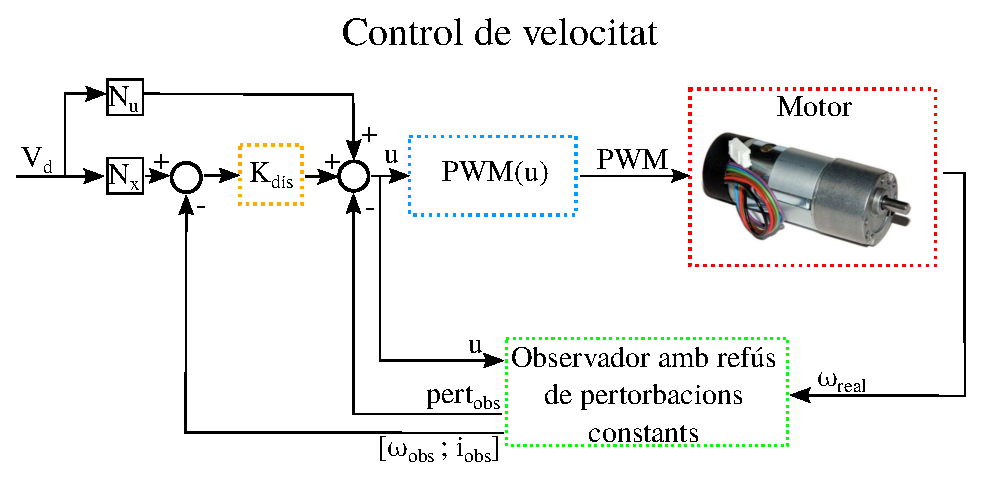
\includegraphics[width=0.8\textwidth]{Imatges/controlVelocitat.eps}
\caption{Esquema del control de velocitat\label{fig:controlVelocitat}}
\end{figure}

\newpage
Per últim, es presenta a continuació, figura \ref{fig:controlVelocitatGraph}, una comparativa de les velocitats que assoleix el motor en un tram de temps determinat. Aquí es poden observar un parell de fets. Per una banda, encara que tots els pols de llaç tancat del control siguin reals, aquí apareixen sobrepuigs típics dels pols complexos. Una explicació possible d'això és que el sistema conté zeros i, aquests poden provocar aquest tipus de comportament. Per altra banda, també s'observen pics esporàdics que, fins i tot, sobrepassen el rang de velocitats de treball del motor. A més, aquest pic és tant de la velocitat real mesurada, com de l'observada. L'explicació que és veu d'això és que la mesura de la velocitat en alguns moments falla i l'observador en tenir una resposta tan ràpida, segueix aquest error. Per tant, dues formes de solventar-ho podrien ser corregir la mesura de la velocitat de tal forma que fos més robusta i utilitzar uns pols de llaç tancat de l'observador més lents.

\begin{figure}[h]
\centering
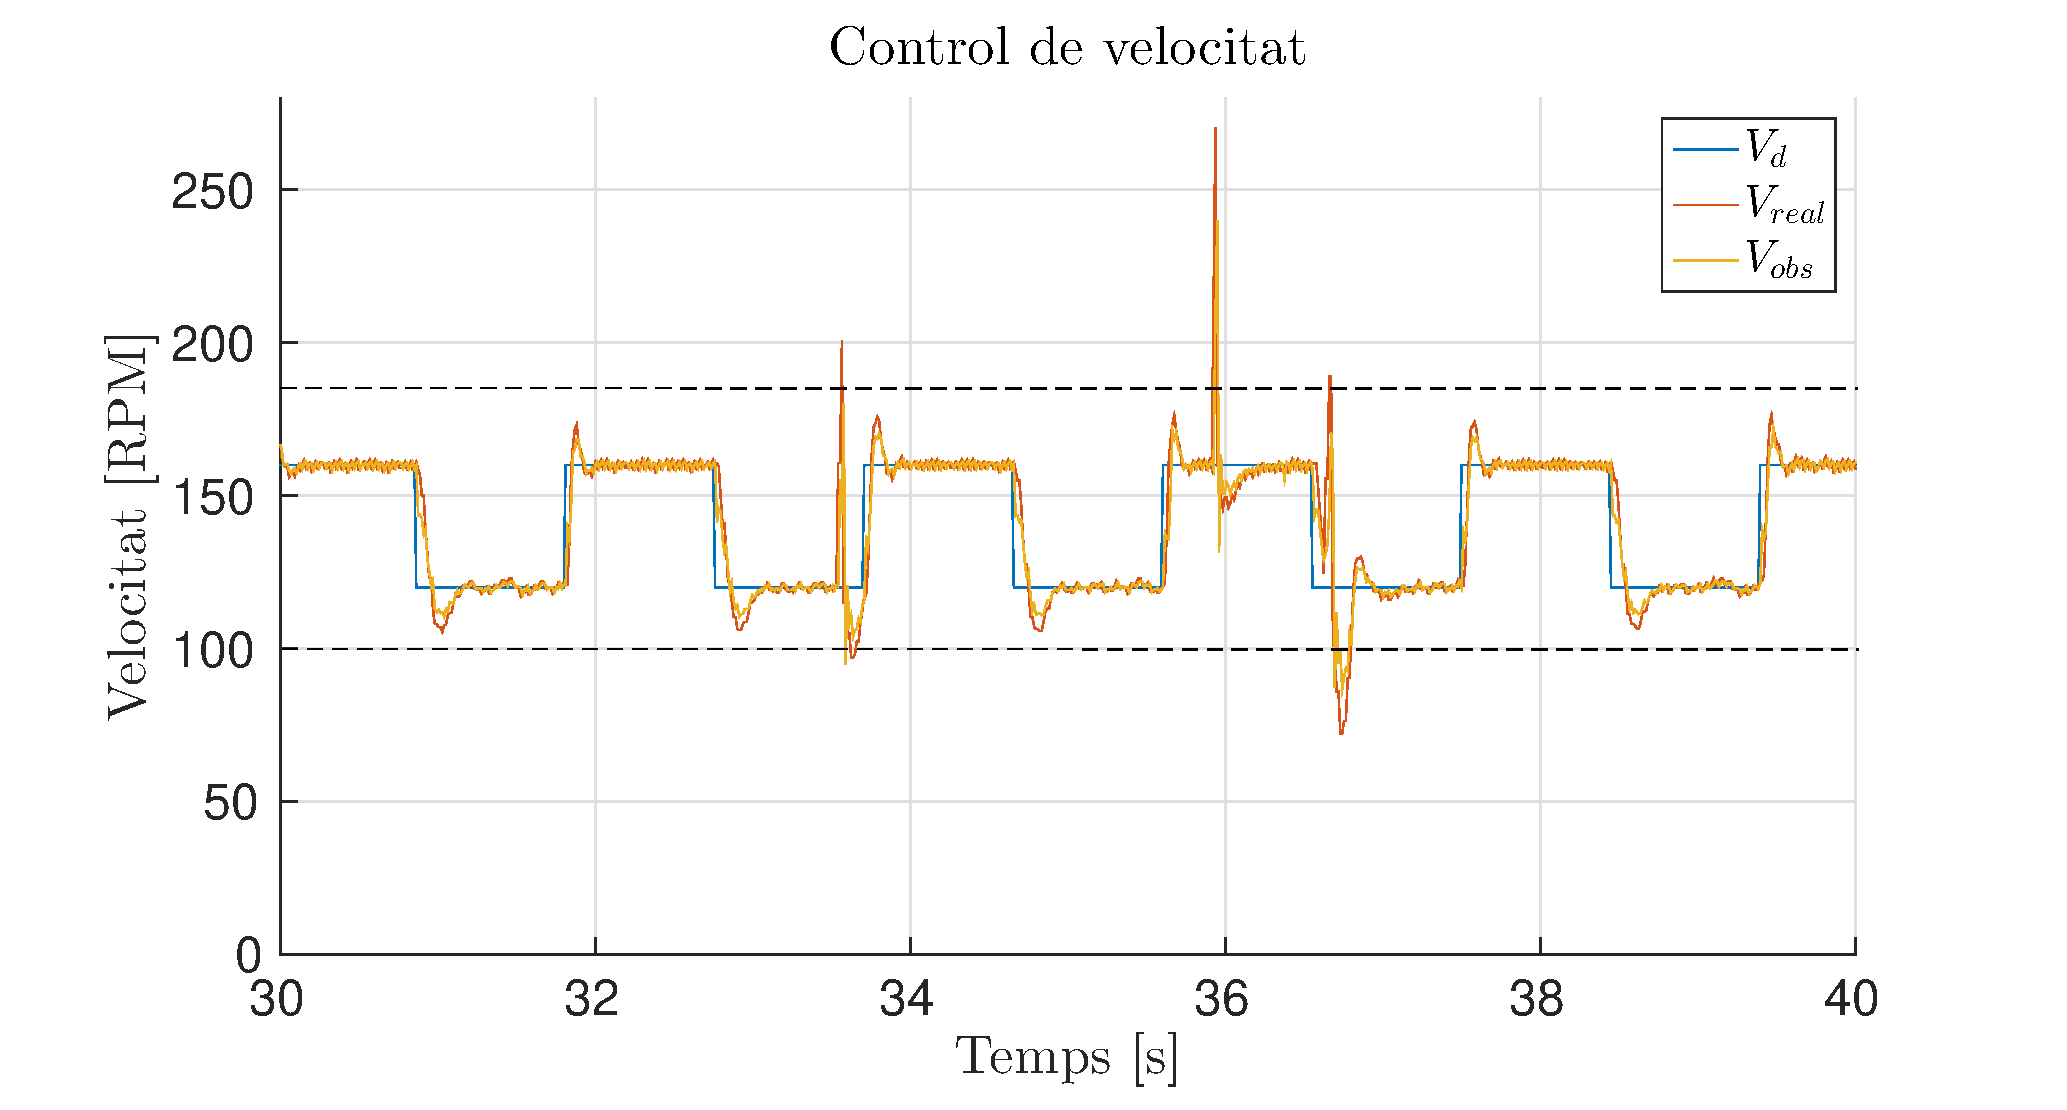
\includegraphics[width=0.8\textwidth]{Imatges/controlVelocitatGraph.eps}
\caption{Dades de les diferents velocitats en un tram determinat. Marcat en discontinua el rang de velocitats on treballa realment el motor.\label{fig:controlVelocitatGraph}}
\end{figure}

\section{Control de posició}

El control de posició el que permet és donada una referència de posició, el motor va a aquesta. Aquest tipus de funcionament és el mateix que inclou un servomotor, per tant, es pot considerar que amb aquest control s'estaria aconseguint que un motor DC barat funcionés com un servomotor.

Per dur a terme el control s'ha de modificar el model del que es partia. Ara s'ha d'incloure la variable d'estat de la posició on la seva derivada és la velocitat. Per tant, el model queda representat com en l'equació \eqref{eq:modelPos_teoric1}. Amb aquest model es pot observar com, realment, s'està afegint un integrador al llaç obert. Per tant, dur a terme el control amb refús de pertorbacions constants no tindria sentit ja que s'estaria posant un pol doble al $0$ (en continu), provocant així la inestabilitat d'una planta que de per sí és estable.

\begin{equation}
\frac{d}{dt}\begin{bmatrix}
\theta\\
\dot{\theta}\\
i
\end{bmatrix} = \begin{bmatrix}
0 & 1 & 0\\
0 & -\frac{b}{J} & \frac{K}{J}\\
0 & -\frac{K}{L} & -\frac{R}{L}
\end{bmatrix}
\begin{bmatrix}
\theta\\
\dot{\theta}\\
i
\end{bmatrix} + \begin{bmatrix}
0\\
0\\
\frac{1}{L}
\end{bmatrix} V \label{eq:modelPos_teoric1}
\end{equation}

En un primer moment, es podria pensar que per aquest observador tant es podria fer observant la velocitat, $C=\begin{bmatrix}0 & 1 & 0\end{bmatrix}$ com la posició, $C =\begin{bmatrix}1 & 0 & 0\end{bmatrix}$. Ara bé, si es du a terme l'estudi d'observabilitat, observable si $\begin{bmatrix}C\\CA\\CA^2\end{bmatrix}$ és de rang complert, pels dos casos, es comprova com només es pot dur a terme l'observador a partir de la posició. Per tant, al model, de l'equació \eqref{eq:modelPos_teoric1}, se li afegeix la sortida de l'equació \eqref{eq:modelPos_teoric2}.

\begin{equation}
y = \begin{bmatrix}
1 & 0 & 0
\end{bmatrix} \begin{bmatrix}
\theta\\
\dot{\theta}\\
i
\end{bmatrix}\label{eq:modelPos_teoric2}
\end{equation}

A l'hora de treballar amb el control de posició s'ha d'utilitzar un control amb observació, amb la posició real com a variable d'estat observada, que s'extreu com s'ha explicat en la introducció de l'informe. Per tant, aquí el que s'ha d'implementar és el càlcul de la posició real, juntament amb un sistema que permeti el canvi de sentit del motor en el moment en que l'acció de control sigui negativa.

Amb l'explicació donada just a sobre, sembla com si el control de posició hagués de ser senzill, però no ho és ja que al llarg de l'experiència sorgeixen diferents inconvenients que dificulten la tasca. Per una banda, la implementació de la mesura de la posició dona cert problemes que ara encara no s'han pogut arribar a solventar i, per tant, la implementació del control de posició ja no és factible.

\chapter{Conclusions}

Com a conclusions sobre la identificació i el control del motor destacar el fet d'haver-se quedat amb les ganes d'aconseguir dur a terme el control de posició, tot i dedicar-hi hores al final del curs no s'han solventat tots els problemes. Per altra banda, destacar que es nota la diferència de quan el model et ve donat a quan el comences des de zero i t'has d'espavilar per poder arribar a fer un bon model per després no tenir problemes en el control, a més d'estar utilitzant uns sensors que tenen mala precisió. 

Afegir que en aquest informe es poden pensar com a treballs futurs l'ús d'interrupcions de \textit{Timer} o l'ús de \textit{Real-Time}, tant per extreure el model, com pel control en sí. També, es podria plantejar l'estudi sobre els diferents pols de llaç tancat que poden donar una bona resposta. Per últim, també es pot mirar de plantejar diferents valors inicials dels paràmetres del model, a l'hora de minimitzar la distància, per comprovar si es poden trobar altres òptims que donin valors més realistes.

Com experiència, m'ha semblat molt enriquidora, ja que per fi m'he trobat amb els problemes que es tenen en el dia a dia quan es fa control, i he aprés sobre aquests. A més, m'ha motivat molt la forma de treballar i crec que s'hauria de fer més sovint així.
\end{document}
